\documentclass{beamer}  
\usetheme{Berkeley}
\usepackage{lipsum}
\usepackage{graphicx}
%%%%%%%%%%%%%%%%%%%%%%%%%%%%%%%%%%%%%%%%

\title[This ``short title'' is clearly way too long, don't you think?]{Improving on 97th-order Edgeworth Expansions for the Mean of a Normal Population}
\author[Hyde \& Nosferatu]{Jekyll N.\ Hyde\inst{1,3}  \and Archibald W.\ Nosferatu\inst{2}}
\institute[UTran]{\inst{1} Center for the Study of Dark Arts, University of Transylvania, \and %
                      \inst{2} Transylvania Federal Reserve Bank \and %
                      \inst{3} NBER} 

\date{November 18th, 2018}

\begin{document} 

\maketitle
%%%%%%%%%%%%%%%%%%%%%%%%%%%%%%%%%%%%%%%%
\section{This is a really long section title}
\begin{frame}
  \frametitle{Literature Review: wherein the speaker wastes 5 minutes citing irrelevant work with no context.} 
  \begin{itemize}
    \item Statistics: Bayes \& Price (1768), Gauss (1810), Laplace (1820), Student (1908), Fisher (1930,1931, 1932, 1935, 1955), Neyman (1958, 1959, 1961, 1962)
    \item Economics: Smith (1776), Ricardo (1817), Marx (1867, 1885, 1894), Marshall (1890), Keynes (1938), Schumpeter (1942), Samuelson (1948), Mas-Colell et al.\ (1995)
    \item English Literature: Beowulf (700--1000), The Canterbury Tales (1400), The Faerie Queene (1590), The Winter's Tale (1623), Pride and Prejudice (1813), Vanity Fair (1848), For Whom the Bell Tolls (1940) 
    \item Popular Films: Casablanca (1942), Sunset Boulevard (1950), Jaws (1975), Star Wars (1977, 1980, 1983), E.T.\ (1982), Titanic (1997), Harry Potter (2001, 2002, 2004, 2005, 2007, 2009, 2010, 2011) 
  \end{itemize}
\end{frame}

%%%%%%%%%%%%%%%%%%%%%%%%%%%%%%%%%%%%%%%%
\section{This one is also long}
\begin{frame}
  \frametitle{A Table: wherein the speaker and audience pretend that they have any idea what these numbers mean.}

  \tiny
  \begin{tabular}{llll}
    \hline \hline
    Design \#1 & Design \#2 & Design \#3 & Design \#4\\
    \hline
     1.23456789009876554 & 1.23456789009876554 & 1.23456789009876554 & 1.23456789009876554\\
     1.23456789009876554 & 1.23456789009876554 & 1.23456789009876554 & 1.23456789009876554\\
     1.23456789009876554 & 1.23456789009876554 & 1.23456789009876554 & 1.23456789009876554\\
     1.23456789009876554 & 1.23456789009876554 & 1.23456789009876554 & 1.23456789009876554\\
     1.23456789009876554 & 1.23456789009876554 & 1.23456789009876554 & 1.23456789009876554\\
     1.23456789009876554 & 1.23456789009876554 & 1.23456789009876554 & 1.23456789009876554\\
     1.23456789009876554 & 1.23456789009876554 & 1.23456789009876554 & 1.23456789009876554\\
     1.23456789009876554 & 1.23456789009876554 & 1.23456789009876554 & 1.23456789009876554\\
     1.23456789009876554 & 1.23456789009876554 & 1.23456789009876554 & 1.23456789009876554\\
     1.23456789009876554 & 1.23456789009876554 & 1.23456789009876554 & 1.23456789009876554\\
     1.23456789009876554 & 1.23456789009876554 & 1.23456789009876554 & 1.23456789009876554\\
     1.23456789009876554 & 1.23456789009876554 & 1.23456789009876554 & 1.23456789009876554\\
     1.23456789009876554 & 1.23456789009876554 & 1.23456789009876554 & 1.23456789009876554\\
     1.23456789009876554 & 1.23456789009876554 & 1.23456789009876554 & 1.23456789009876554\\
     1.23456789009876554 & 1.23456789009876554 & 1.23456789009876554 & 1.23456789009876554\\
     1.23456789009876554 & 1.23456789009876554 & 1.23456789009876554 & 1.23456789009876554\\
     1.23456789009876554 & 1.23456789009876554 & 1.23456789009876554 & 1.23456789009876554\\
     1.23456789009876554 & 1.23456789009876554 & 1.23456789009876554 & 1.23456789009876554\\
     1.23456789009876554 & 1.23456789009876554 & 1.23456789009876554 & 1.23456789009876554\\
     1.23456789009876554 & 1.23456789009876554 & 1.23456789009876554 & 1.23456789009876554\\
     1.23456789009876554 & 1.23456789009876554 & 1.23456789009876554 & 1.23456789009876554\\
     1.23456789009876554 & 1.23456789009876554 & 1.23456789009876554 & 1.23456789009876554\\
     1.23456789009876554 & 1.23456789009876554 & 1.23456789009876554 & 1.23456789009876554\\
     1.23456789009876554 & 1.23456789009876554 & 1.23456789009876554 & 1.23456789009876554\\
     1.23456789009876554 & 1.23456789009876554 & 1.23456789009876554 & 1.23456789009876554\\
     1.23456789009876554 & 1.23456789009876554 & 1.23456789009876554 & 1.23456789009876554\\
     1.23456789009876554 & 1.23456789009876554 & 1.23456789009876554 & 1.23456789009876554\\
     1.23456789009876554 & 1.23456789009876554 & 1.23456789009876554 & 1.23456789009876554\\
     1.23456789009876554 & 1.23456789009876554 & 1.23456789009876554 & 1.23456789009876554\\
     1.23456789009876554 & 1.23456789009876554 & 1.23456789009876554 & 1.23456789009876554\\
    \hline
  \end{tabular}

\end{frame} 
%%%%%%%%%%%%%%%%%%%%%%%%%%%%%%%%%%%%%%%%
\section{This one is shorter}
\begin{frame}
  \frametitle{If you're too lazy to make a new figure for your talk, why not just distort the one from your paper?}

  \begin{figure}
    \centering
    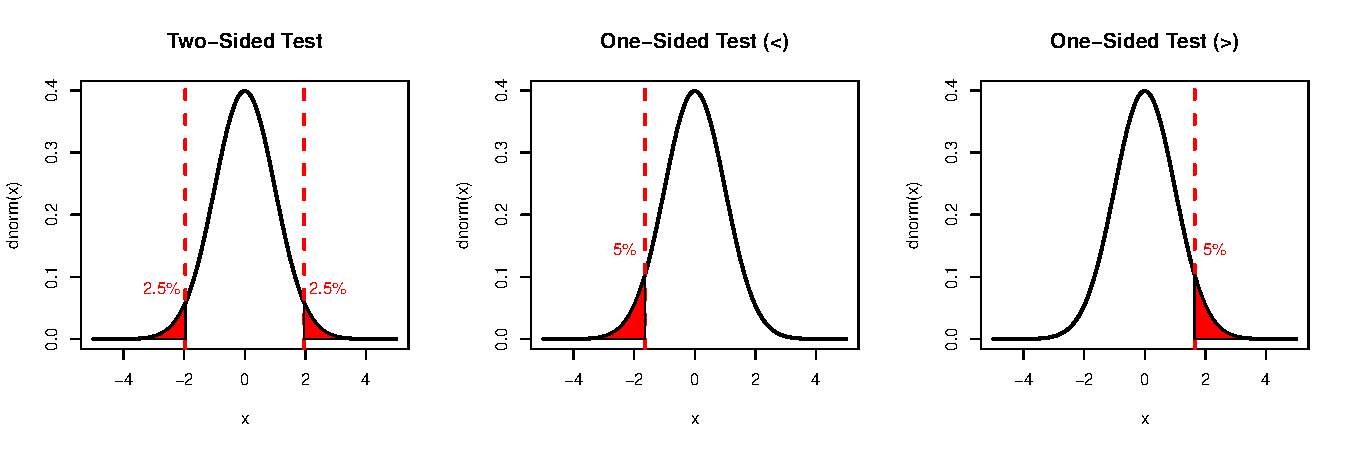
\includegraphics[width=4in,height=3.5in]{onesided_vs_twosided.pdf}
  \end{figure}

\end{frame} 
%%%%%%%%%%%%%%%%%%%%%%%%%%%%%%%%%%%%%%%%
\section{This one is shorter}
\begin{frame}
  \frametitle{Isn't it fun to write titles that are overly-long, convey no information, and distract the audience?}
    \scriptsize
  \begin{itemize}
    \item \lipsum[1]
    \item \lipsum[2]
  \end{itemize}
\end{frame} 
%%%%%%%%%%%%%%%%%%%%%%%%%%%%%%%%%%%%%%%%
\section{Is this even necessary? Why are we bothering?}
\begin{frame}
  \frametitle{Some Final (Bad) Advice}
To really impress the audience, take more than your allotted time but nevertheless rush through the last 20 slides\ldots 
\end{frame} 
%%%%%%%%%%%%%%%%%%%%%%%%%%%%%%%%%%%%%%%%
\end{document}
